\chapter{Metric learning}


\begin{description}
    \item[Metric learning] \marginnote{Metric learning}
        Task of training a network that produces discriminative embeddings (i.e., with a clustered structure) such that:
        \begin{itemize}
            \item The distance of related objects (i.e., intra-class distance) is minimized.
            \item The distance of different objects (i.e., inter-class distance) is maximized.
        \end{itemize}
\end{description}

\section{Face recognition}

\begin{description}
    \item[Face recognition] \marginnote{Face recognition}
        Given a database of identities, classify a query face.

        \begin{description}
            \item[Open-world setting]
                System where it is easy to add or remove identities.
        \end{description}
\end{description}


\subsection{Face recognition as classification}

\begin{description}
    \item[Plain classifier] \marginnote{Plain classifier}
        Consider each identity as a class and use a CNN with a softmax head to classify the input image.

        \begin{remark}
            This approach requires a large softmax and do not allow adding or removing identities without retraining.
        \end{remark}

    \item[kNN classifier] \marginnote{kNN classifier}
        Use a feature extractor to embed faces and use a kNN classifier to recognize it.

        \begin{description}
            \item[Gallery] \marginnote{Gallery}
                Set of embeddings of known identities.
        \end{description}

        \begin{remark}
            This approach allows to easily add or remove new identities.
        \end{remark}

        \begin{figure}[H]
            \centering
            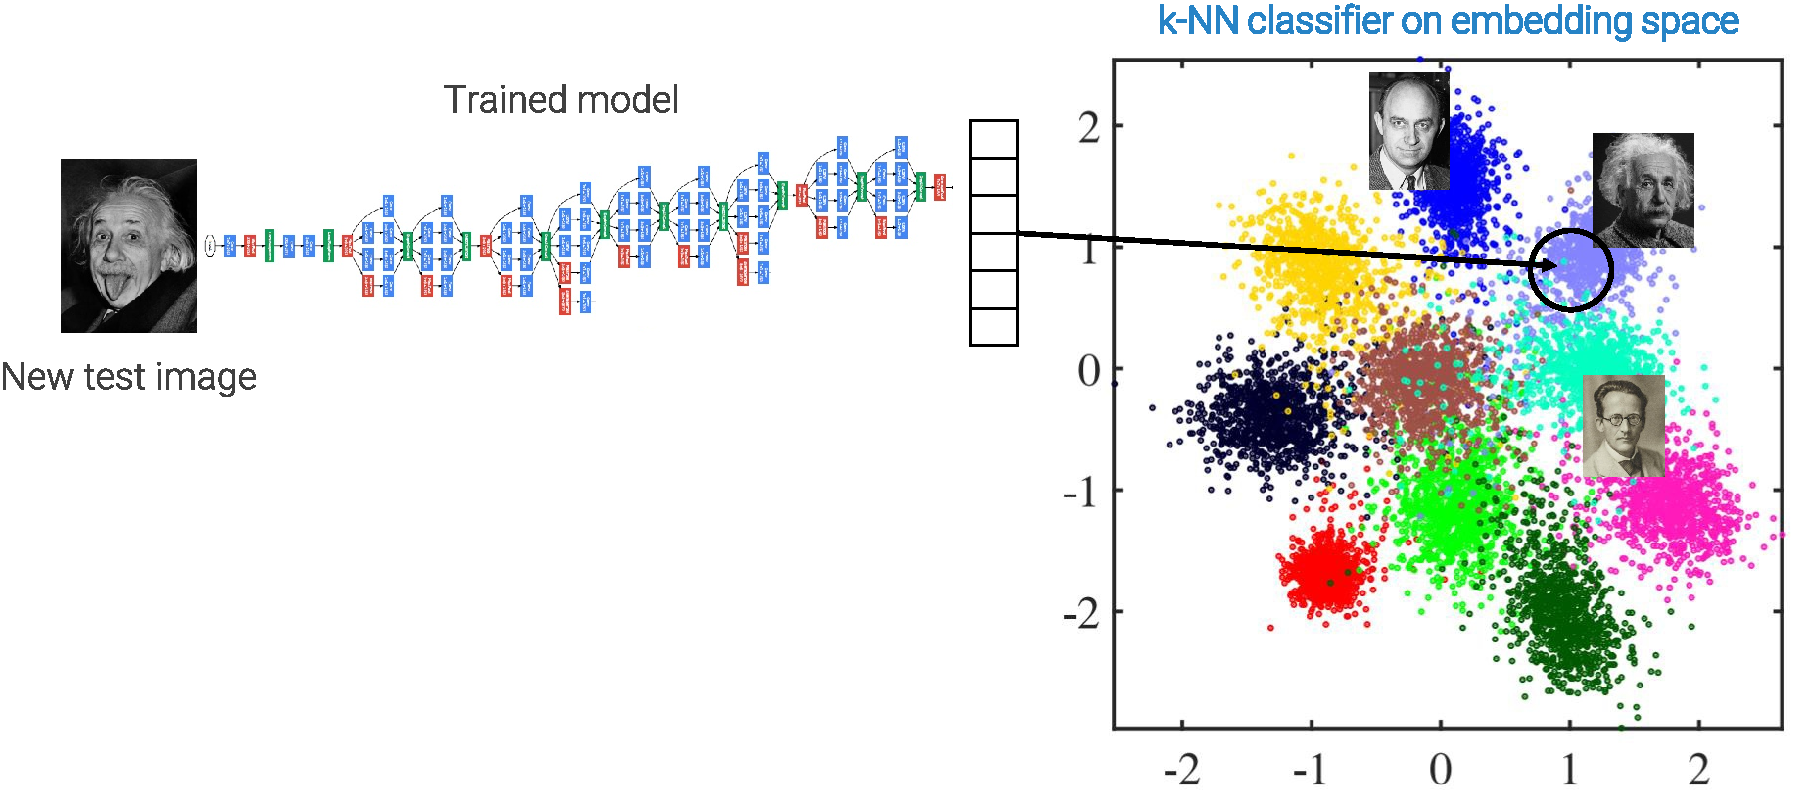
\includegraphics[width=0.7\linewidth]{./img/_cnn_knn_face_recognition.pdf}
        \end{figure}

        \begin{remark}
            Feature extractors for classification are trained using the cross-entropy loss to learn semantically rich embeddings. However, when classifying, these embeddings are passed through a final linear layer. Therefore, it is sufficient that they are linearly separable.

            In other words, the distance between elements of the same class can be arbitrarily large and the distance between different classes can be arbitrarily small, as long as they are linearly separable.

            \begin{figure}[H]
                \centering
                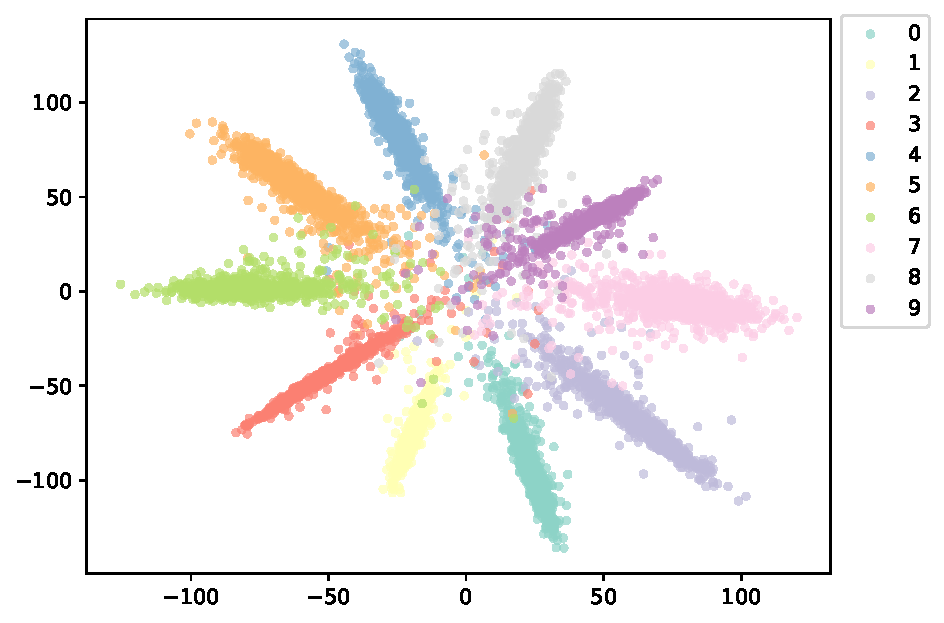
\includegraphics[width=0.45\linewidth]{./img/_mnist_embeddings.pdf}
                \caption{MNIST embeddings in 2D}
            \end{figure}
        \end{remark}
\end{description}


\section{Face verification}

\begin{description}
    \item[Face verification] \marginnote{Face verification}
        Task of confirming that two faces represent the same identity. This problem can be solved by either:
        \begin{itemize}
            \item Using better metrics than the Euclidean distance (e.g., as done in DeepFace).
            \item Using better embeddings (e.g., as done in DeepID or FaceNet).
        \end{itemize}

        \begin{remark}
            This task can be used to solve face recognition.
        \end{remark}
\end{description}


\begin{description}
    \item[Siamese network training] \marginnote{Siamese network training}
        Train a network by comparing its outputs from two different inputs. This can be virtually seen as training two copies of the same network with shared weights.

        \begin{figure}[H]
            \centering
            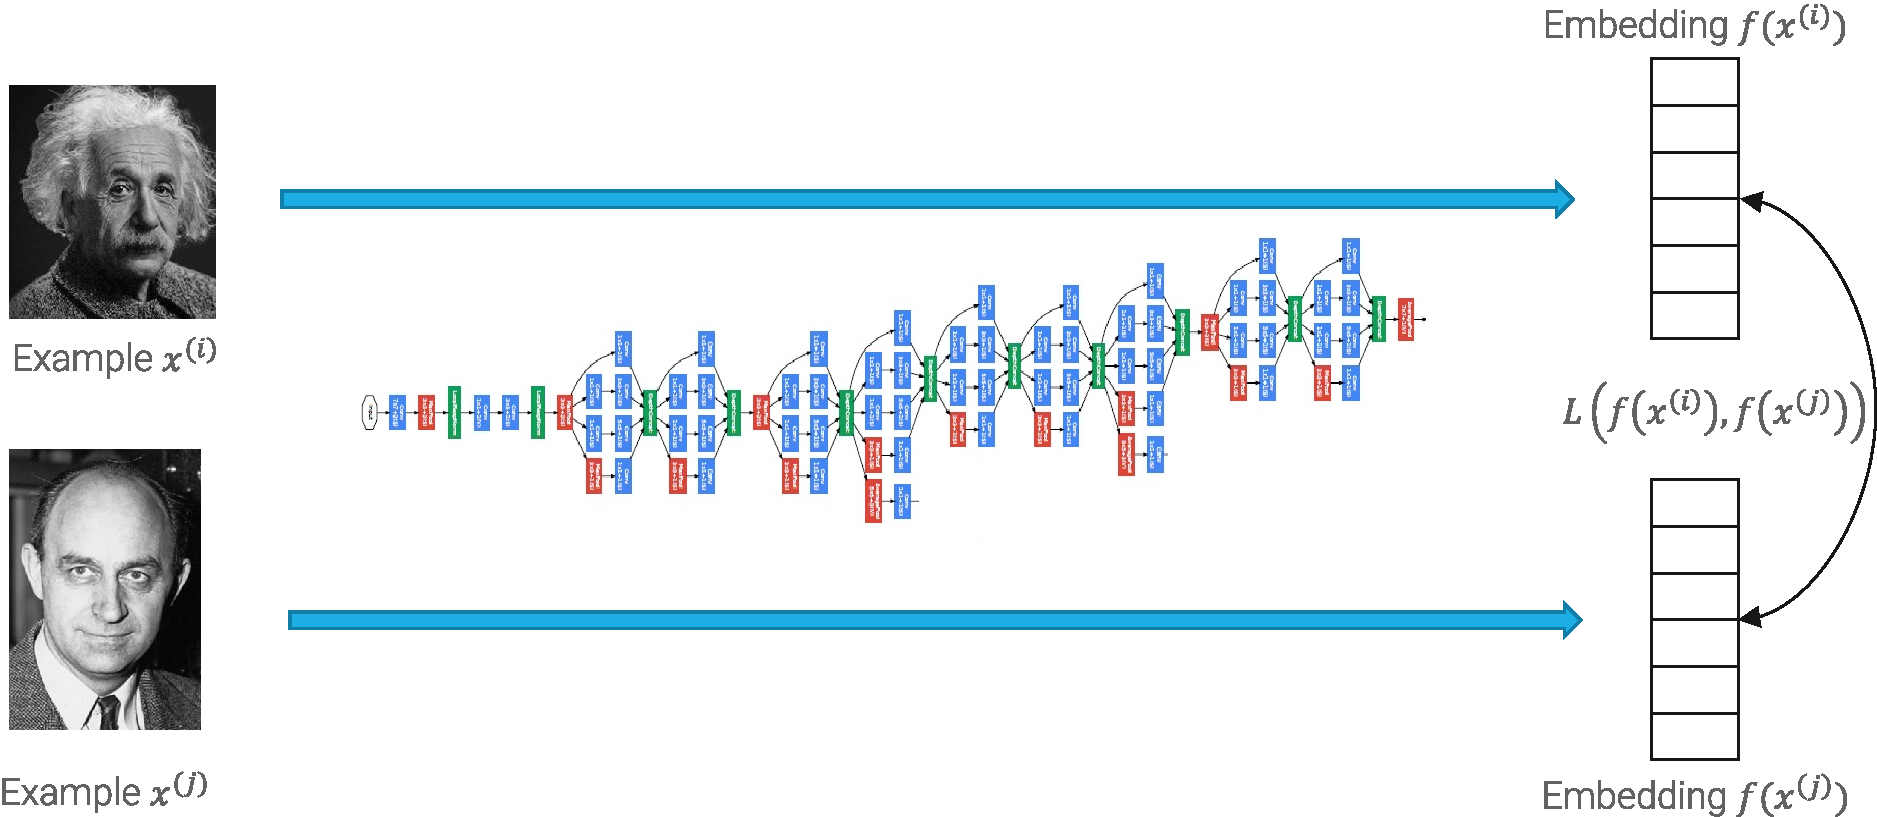
\includegraphics[width=0.7\linewidth]{./img/_siamese_network.pdf}
        \end{figure}

        \item[Contrastive loss] \marginnote{Contrastive loss}
            Loss to enforce clustered embeddings. It is defined as follows:
            \[
                \mathcal{L}\left( f(x^{(i)}), f(x^{(j)}) \right) = 
                \begin{cases}
                    \Vert f(x^{(i)}) - f(x^{(j)}) \Vert_2^2 & \text{if $y^{(i, j)} = +1$ (i.e., same class)} \\
                    - \Vert f(x^{(i)}) - f(x^{(j)}) \Vert_2^2 & \text{if $y^{(i, j)} = 0$} \\
                \end{cases}
            \]
            As the second term is not lower-bounded (i.e., it can be arbitrarily small), a margin $m$ is included to prevent pushing different classes too far away:
            \[
                \begin{split}
                    &\mathcal{L}\left( f(x^{(i)}), f(x^{(j)}) \right) = 
                    \begin{cases}
                        \Vert f(x^{(i)}) - f(x^{(j)}) \Vert_2^2 & \text{if $y^{(i, j)} = +1$} \\
                        \max\left\{0, m - \Vert f(x^{(i)}) - f(x^{(j)}) \Vert_2\right\}^2 & \text{if $y^{(i, j)} = 0$} \\
                    \end{cases} \\
                    &= y^{(i, j)} \Vert f(x^{(i)}) - f(x^{(j)}) \Vert_2^2 + (1-y^{(i, j)}) \max\left\{0, m - \Vert f(x^{(i)}) - f(x^{(j)}) \Vert_2\right\}
                \end{split}
            \]

            \begin{remark}
                A margin $m^+$ can also be added to the positive branch to prevent collapsing all embeddings of the same class to the same point.
            \end{remark}

            \begin{remark}
                The negative branch $\max\left\{0, m - \Vert f(x^{(i)}) - f(x^{(j)}) \Vert_2\right\}$ is the hinge loss, which is used in SVM.
            \end{remark}

            \begin{remark}
                With L2 regularization, the fact that the second term is not lower-bounded is not strictly a problem as the weights lay on a hyper-sphere and therefore set a bound to the output. Still, there is no need to push the embeddings excessively far away.
            \end{remark}
\end{description}